\chapter{Result and discussion}

\section{SAC agent}

In order to solve the helicopter environment, as presented in the previous chapter, we implemented the SAC algorithm. In this section, we have provided the implementation of the soft actor-critic as a controller for the helicopter which is shown in figure \ref{SAC_controller}. We have implemented 5 other reinforcement learning methods such as D4PG \cite{barth2018distributed}, proximal policy optimization (PPO) \cite{schulman2017proximal}, Trust Region Policy Optimization (TRPO) \cite{DBLP:journals/corr/SchulmanLMJA15}, deep deterministic policy gradient \cite{silver2014deterministic} and Twin Delayed DDPG \cite{fujimoto2018addressing} and we were unable to find an stabilized performance of the helicopter using the aforementioned algorithms.

For this study, we use garage \cite{garage} as an API for the agent. Garage implements state-of-the-art deep
reinforcement learning algorithms in Python and coherently integrates with the deep learning
library PyTorch \cite{NEURIPS2019_9015} and Tensorflow \cite{tensorflow2015-whitepaper}. The library provides a straightforward approach to evaluate and test different algorithms in Gym environments. The schematic of agent-environment interaction is illustrated in Figure \ref{SAC_controller}.


\begin{figure} 
	\centering
	\begin{tikzpicture}[auto,node distance=2cm,scale=1.0]
		\node [block,fill=gray!20,](Xd){$X_d$};
		\node [input, right of=Xd, node distance=3cm](sum1){};
		\node [block, fill=gray!20, right of=sum1, node distance=3cm](SAC){SAC agent};
		\node [block, fill=gray!20, right of=SAC, node distance=6cm](plant){Helicopter};
		\node [sum, fill=gray!20, below of=sum1, distance=7m](ypos){-};
		\node [input, below of=sum1](belowsum){};
		\node [input, right of=sum1,node distance=1cm](rightsum){};
		\node [output, right of=plant](out1){};
		\node [output, below of=out1](out2){};
		\draw [arrow] (SAC)--node{$A(t)$}(plant);
		\draw [line] (plant)|- node [pos=0.90]{$X(t)$} (ypos);
		\draw [arrow] (Xd)|-(ypos);
		\draw [arrow] (ypos)|-node[pos=0.80]{$S(t)$}(SAC);
	\end{tikzpicture}
	\caption{SAC controller schematic}
	\label{SAC_controller}
\end{figure}

\subsection{Architecture}

In this section, we discuss the architecture of the SAC actor and critic neural network.

\subsubsection*{Actor}

The actor diagram and schematic of this SAC agent is given in figures \cref{actor_diagram,nnschematic} which includes 2 hidden layer of size 128 and 128 fully connected layers with a Rectified Linear Unity (RelU) activation function and a $tanh$ activation function at last in order to narrow the result to [-1,1], the actions are then linearly mapped to the action range based on the environment\footnote{check action wrapper at Appendix A}. In order to constraint the standard deviation of the policy, it is set to be between $[e^{-20},e^{1}]$.

\begin{figure} 
	\centering
	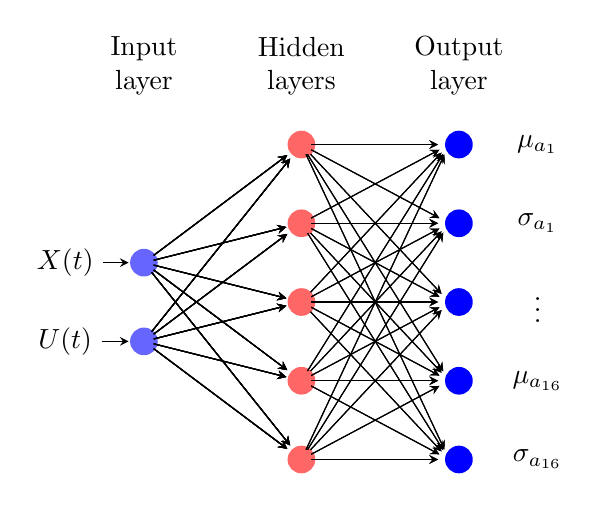
\begin{tikzpicture}[every node/.style={align=center}]
		\foreach \x in{1,2,3,4,5}
		\fill[red!60](0,\x)circle(5pt)node(a\x){};
		
		\fill[blue!60](-2,2.5)circle(5pt)node(b3){};
		\fill[blue!60](-2,3.5)circle(5pt)node(b4){};
		\fill[blue](2,2)circle(5pt)node(c1){};
		\fill[blue](2,3)circle(5pt)node(c2){};
		\fill[blue](2,4)circle(5pt)node(c3){};
		\fill[blue](2,5)circle(5pt)node(c4){};
		\fill[blue](2,1)circle(5pt)node(c5){};
		\node(y4)at(-3,3.5){$X(t)$};
		\node(y3)at(-3,2.5){$U(t)$};
		
		
		\node at(-2,6){Input\\layer};
		\node at(0,6){Hidden\\layers};
		\node at(2,6){Output\\layer};
		\node(d4)at(3,5){$\mu_{a_1}$};
		\node(d3)at(3,4){$\sigma_{a_1}$};
		\node(d2)at(3,3){$\vdots $};
		\node(d1)at(3,2){$\mu_{a_{16}}$};
		\node(d5)at(3,1){$\sigma_{a_{16}}$};
		\foreach \x in{3,4}
		\draw[-{stealth[sep=2pt]}](y\x)--(b\x);
		\foreach \x in{3,4}
		{\foreach \y in{1,2,3,4,5}
			\foreach \z in {1,2,3,4,5}
			{
				{\draw[-{stealth[sep=2pt]}](b\x)--(a\y);
					\draw[-{stealth[sep=4pt]}](a\y)--(c\z.west);
				}
			}
			c}
	\end{tikzpicture}
	\caption{Actor diagram for SAC agent, the inputs are the 16 states of the helicopter $X(t)$ and the 4 control inputs $U(t)$, the outputs are the average $\mu$ and the standard deviation $\sigma$ of the agent actions}
	\label{actor_diagram}
\end{figure}

\subsubsection*{Critic}

The diagram for the Critic neural network is depicted in \cref{critic_diagram,nnschematic}.
The diagram includes 2 hidden layer of size 256 and 256 fully connected layers with RelU activation function after each hidden layers.

\begin{figure} 
	\centering
	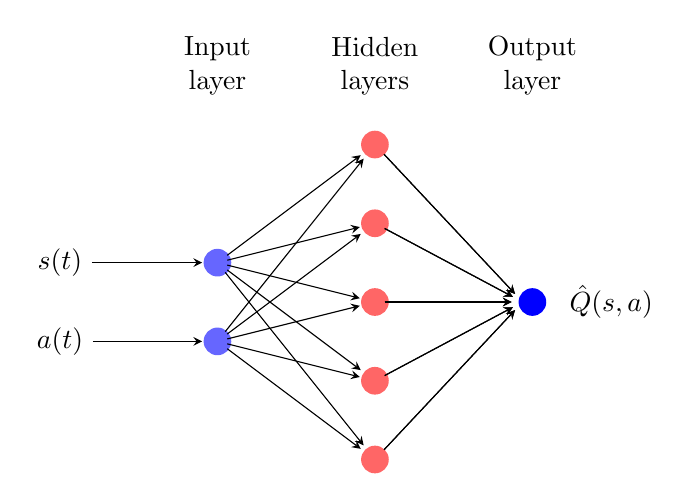
\begin{tikzpicture}[every node/.style={align=center}]
		\foreach \x in{1,2,3,4,5}
		\fill[red!60](0,\x)circle(5pt)node(a\x){};
		\fill[blue!60](-2,2.5)circle(5pt)node(b1){};
		\fill[blue!60](-2,3.5)circle(5pt)node(b2){};
		\fill[blue](2,3)circle(5pt)node(c1){};
		\node(y2)at(-4,3.5){$s(t)$};
		\node(y1)at(-4,2.5){$a(t)$};
		\node at(-2,6){Input\\layer};
		\node at(0,6){Hidden\\layers};
		\node at(2,6){Output\\layer};
		
		\node(d1)at(3,3){$\hat{Q}(s,a)$};
		
		\foreach \x in{1,2}
		\draw[-{stealth[sep=2pt]}](y\x)--(b\x);
		\foreach \x in{1,2}
		{\foreach \y in{1,2,3,4,5}
			\foreach \z in {1}
			{
				{\draw[-{stealth[sep=2pt]}](b\x)--(a\y);
					\draw[-{stealth[sep=4pt]}](a\y)--(c\z.west);
				}
			}
			c}
	\end{tikzpicture}
	\caption{Critic diagram for SAC agent, inputs are the states and actions while the output is the Q value for the given input.}
	\label{critic_diagram}
\end{figure}

\begin{figure} 
	\centering
	\begin{tikzpicture}[auto,node distance=2.5cm,scale=0.4]
		\node [block,fill=gray!20,](firstlayer){linear: $\rightarrow 128$};
		\node [below of=firstlayer](input){observations};
		\node [block, fill=gray!20, above of=firstlayer, node distance=2.5cm](secondlayer){linear: $\rightarrow$ 128};
		\node [block, above of=secondlayer, node distance=2.5cm](thirdlayer){linear: $\rightarrow$ 32};
		\node [above of=thirdlayer, node distance=2.5cm](actions){actions};
		
		
		\node [block, right of= firstlayer,fill=gray!20,node distance=7cm](flayercritic){linear: $\rightarrow 256$};
		\node [below of=flayercritic](criticinput){observation and actions};
		\node [block, fill=gray!20, above of=flayercritic, node distance=2.5cm](slayercritic){linear: $\rightarrow$ 256};
		\node [block, above of=slayercritic, node distance=2.5cm](thlayercritic){linear: $\rightarrow$ 1};
		\node [above of=thlayercritic, node distance=2.5cm](atoms){$\hat{Q}$};
		
		\draw [arrow] (input)--(firstlayer);
		\draw [arrow] (firstlayer)--node[pos=0.30]{$RelU$}(secondlayer);
		\draw [arrow] (secondlayer) --node[pos=0.30]{$RelU$}(thirdlayer);
		\draw [arrow] (thirdlayer) --node[pos=0.30]{$Tanh$}(actions);
		
		\draw [arrow] (criticinput)--(flayercritic);
		
		
		\draw [arrow] (flayercritic)--node[pos=0.30]{$RelU$}(slayercritic);
		\draw [arrow] (slayercritic) --node[pos=0.30]{$RelU$}(thlayercritic);
		\draw [arrow] (thlayercritic) --node[pos=0.20]{}(atoms);
		\node[fit=(firstlayer)(input)(secondlayer)(thirdlayer)(actions),draw,blue,dashed,
		label={[blue]above: actor neural network layers}]{};
		\node[fit=(flayercritic)(criticinput)(slayercritic)(thlayercritic)(atoms),draw,red,dashed,label={[red]above: critic neural network layers}]{};
	\end{tikzpicture}
	\caption{Actor and critic neural network diagram}
	\label{nnschematic}
\end{figure}

\subsection{Hyper-parameters}

Optuna package is utilized for optimization of all the hyperparameters of the SAC agent \cite{optuna_2019}. The SAC agent's primary hyper-parameters are given in table \ref{table of hyperparameters} as part of its implementation.
\begin{longtable}{c|c|c} 
	\caption {Hyper parameters of SAC agent.}\label{table of hyperparameters}\\\toprule
	\endfirsthead
	\caption* {\textbf{Table \ref{table of hyperparameters} Continued:} }\\\toprule
	\endhead
	\endfoot
	\bottomrule
	\endlastfoot
		\textbf{Hyper parameter} & \textbf{Value} & \textbf{description}  \\ \hline \hline
$\mathcal{T}$ & $5\times10^{7}$ &  Total number of environment steps.\\&& \\ \hline
$\mathcal{B}$ & 2048  & mini batch which is the number of samples\\&& from the buffer randomly sampled for each\\&& stochastic gradient decent step update\\&& \\ \hline
$\mathcal{D}$ & $10^7$  &replay buffer size, which is the total number\\&& of steps saved in buffer (when new ones are\\&& added the oldest ones are removed.)\\&& \\ \hline
$\l_{\kappa}$  & $3\times 10^{-4}$  & learning rate for optimization of policy \\&& by this factor.\\&& \\ \hline
$\l_{\delta}$  & $3\times 10^{-4}$  & learning rate for optimization of Q functions.\\&& \\ \hline
$\tau_{target}$  & $5\times 10^{-3}$  & updating the target network linearly\\&& by this factor.\\&& \\ \hline
$\gamma$  & 0.99  &  factor for discounting later rewards.\\&& \\ \hline
$\alpha$  & $3\times e^{-0.009i}$ & the temperature term in SAC policy.\\&& \\ \hline
$\chi$  & $3\times 10^{-3}$  & The learning rate of Adam optimizer.\\&& \\ \hline
$\sigma_{mean}$  & $e^{-20}$  & the minimum standard deviation of the\\&& actions in the stochastic policy of SAC.\\&& \\ \hline
$\sigma_{mean}$  & $e^{1}$  &  the maximum standard deviation of the\\&& actions in the stochastic policy of SAC\\&& \\ \hline
$i_{max}$  & $10^4$  &  the maximum  number of iteration\\&& \\ \hline
\end{longtable}

The replay buffer is designed to contain $10^7$ transition tuples before starting the SAC algorithm. The experience replay buffer enables learning from prior policy experiences while avoiding correlated samples in the gradient step. Furthermore, we implement an upgraded target network with a target factor of $5\times10^{-3}$.This is motivated by the desire to improve the stability of the learning process. Based on line 21 of algorithm \ref{sac algorithm}, if it is time to update, the gradient step  per epoch is set to 2 and the gradient step per iteration is set to 8. For each time a gradient step is executed, a mini-batch of 2048 random samples is chosen from the replay buffer. The learning rate for Adam optimizer on both neural network is set to be $3\times10^{-3}$.

The training of the network included about $5\times10^{7}$ to  $6\times10^{7}$ environment time steps of about 0.03, simulation time. The simulation is run in a 32-cores Intel(R) Xeon(R) CPU E5-2620 v4 @ 2.10GHz which took about 3–4 days.

\section{Results}

\subsection{Training and evaluation}

The training result is given in \ref{ave_return}. The iteration is continued for 10,000 iterations; however, no significant improvement is found after 6000. The standard deviation increases as the number of iterations increases. This is acceptable because at first, in all the episodes, the simulated UAV crashes. However, as the training progresses, the agent improves its action to stabilize the helicopter and hence the difference between the return of points closer to the origin and those placed at a more distant point from the origin grows.

\begin{figure}
	\begin{center}
		\hbox{\hspace*{-2.5cm} 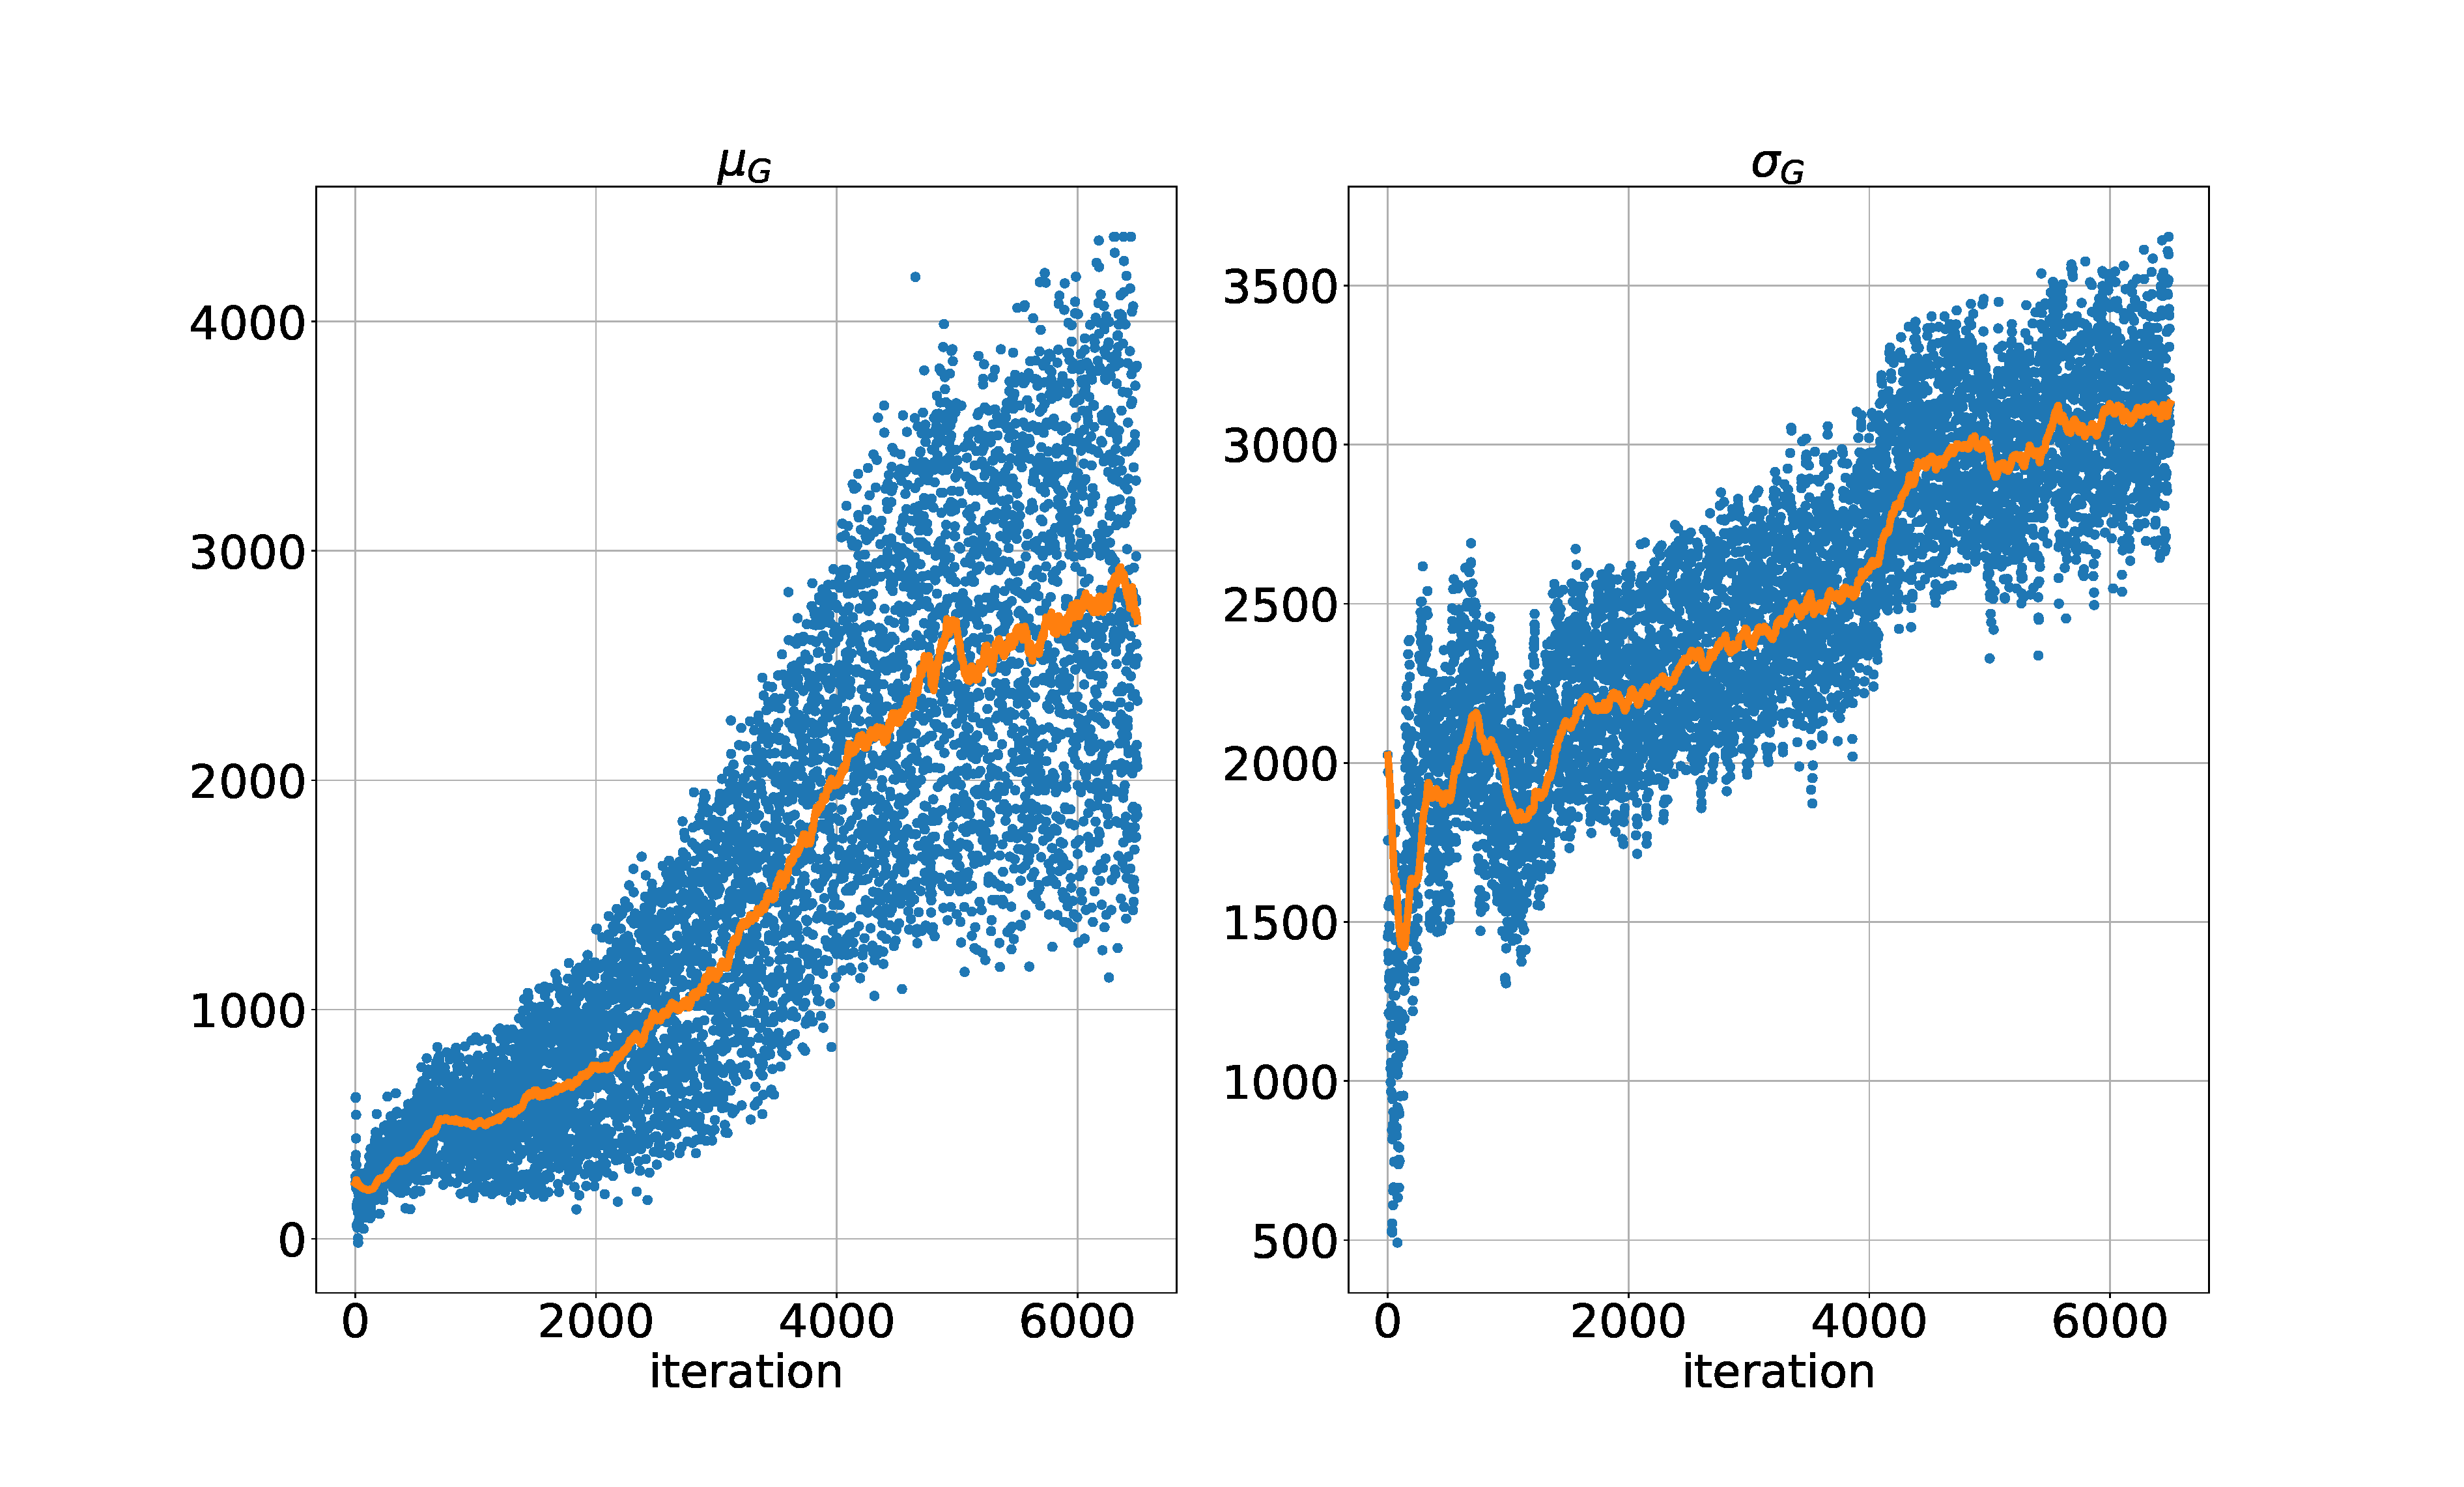
\includegraphics[scale=0.31]{avereturn.eps}}

		\caption{Averaged discounted return $\mu_G$ and standard deviation $\sigma_G$ of each iteration using the random actions of the policy.}
		\label{ave_return}
	\end{center}
\end{figure}

\subsection{Comparison of Controllability and stability to the SMC}

In order to be able to compare the results obtained by an RL method to a traditional control method, the results of controlling the initial point set to [-1,-1,-1] are shown in \cref{states,omega,theta,v_res,actions_delta,flapping} for both the sliding mode controller (SMC) and the SAC policy obtained. As seen, the resulting policy achieves good stabilization capability.

The settling time is considered to be the time when the states reach 0.10 m of the origin which is the desired state. The rise time in this study is considered to be the time for the response to rise from the absolute value of 0.9 m to 0.1 m in the vicinity of origin for each x, y and z states. Considering the aforementioned definitions the comparison between the SAC and SMC is given in table \ref{SAC_SMC}.

\begin{longtable}{c||c|c|c|c} 
	\caption {Comparison of SAC and SMC based on the response characteristics of the helicopter dynamic system for the case of initial point set to [-1,-1,-1].}\label{SAC_SMC}\\\toprule
	\endfirsthead
	\caption* {\textbf{Table \ref{SAC_SMC} Continued:} }\\\toprule
	\endhead
	\endfoot
	\bottomrule
	\endlastfoot
	\textbf{} & \textbf{settling time [s]} & \textbf{rise time [s]} & \textbf{overshoot [m]} & \textbf{SS error [m]}  \\ \hline \hline
	\textbf{x,SMC} & 5.07 & \textbf{0.79} & 0.13 & 0.0  \\ 
	\textbf{x,SAC} & \textbf{4.41} & 3.96 & \textbf{0} & 0  \\ \hline
	
	\textbf{y,SMC} & \textbf{1.36} & \textbf{1.0} & 0.09 & 0.05  \\ 
	\textbf{y,SAC} & 2.96 & 2.66 & \textbf{0} & 0.05  \\ \hline
	
	\textbf{z,SMC} & \textbf{1.51} & \textbf{1.47} & \textbf{0.03} & \textbf{0}  \\ 
	\textbf{z,SAC} & 2.6 & 2.45 & 0.1 & 0.1  \\
	
\end{longtable}

Based on the given comparison result on \ref{SAC_SMC} the sliding mode controller provides a better result in the case of x y and z. The $\psi$ angle has a $10.8^{\circ}$ steady-state error which is not superior to the sliding mode controller ($1.8^{\circ}$). However, it should be mentioned that the sliding mode controller is a highly tuned controller for this system. On the other hand, the SAC agent is a model-free method in which it did not have any access to the model. 

The result of the control input is given in figure \ref{actions_delta}. There are some vibrations in the $\delta_{ped}$ and $\delta_{col}$, We find that it was somewhat hard to reduce these vibrations because as we increased the control derivative input term in the \ref{control_reward}, the policy would alternate between getting closer to the target and achieving a stable hovering somewhere far from the origin. 

\subsubsection {robustness}

In order to test the robustness of the policy, a simulated wind is blown at the UAV given the following equation:

\begin{equation}
	V_{wind,t}=V_{wind,t-1}+ W
\end{equation}

in which W is a random number in [-0.1,0.1] at each time step and using the policy generated. It achieved 100\% stability in all the 27 initial positions, In order to compare the results of the simulation with and without the wind, the rise time, settling time, and steady-state errors are given in table \ref{wind_sac} for the [-1,-1,-1] case.

\begin{longtable}{c||c|c|c|c} 
	\caption {Robustness response characteristics of the helicopter dynamic system  for the SAC policy by a simulated wind for the case of initial point set to [-1,-1,-1].}\label{wind_sac}\\\toprule
	\endfirsthead
	\caption* {\textbf{Table \ref{wind_sac} Continued:} }\\\toprule
	\endhead
	\endfoot
	\bottomrule
	\endlastfoot
	\textbf{} & \textbf{settling time [s]} & \textbf{rise time [s]} & \textbf{overshoot [m]} & \textbf{SS error [m]}  \\ \hline \hline
	\textbf{x} & 4.29 & 3.87 & 0 & 0.03  \\ \hline
	\textbf{y} & 2.87 & 2.57 & 0.08 & 0.02  \\ \hline
	\textbf{z} & 2.47 & 2.36 & 0.09 & 0.09  \\
	
\end{longtable}

\begin{figure}
	\begin{center}
		{\includegraphics[scale=0.41]{X.pdf}}
		\caption{Helicopter SMC and SAC positional states by initial position [-1,-1,-1].}
		\label{states}
	\end{center}
\end{figure}

\begin{figure}
	\begin{center}
		{\includegraphics[scale=0.41]{omega.pdf}}
		\caption{Helicopter SMC and SAC angular velocities by initial position [-1,-1,-1].}
		\label{omega}
	\end{center}
\end{figure}

\begin{figure}
	\begin{center}
		{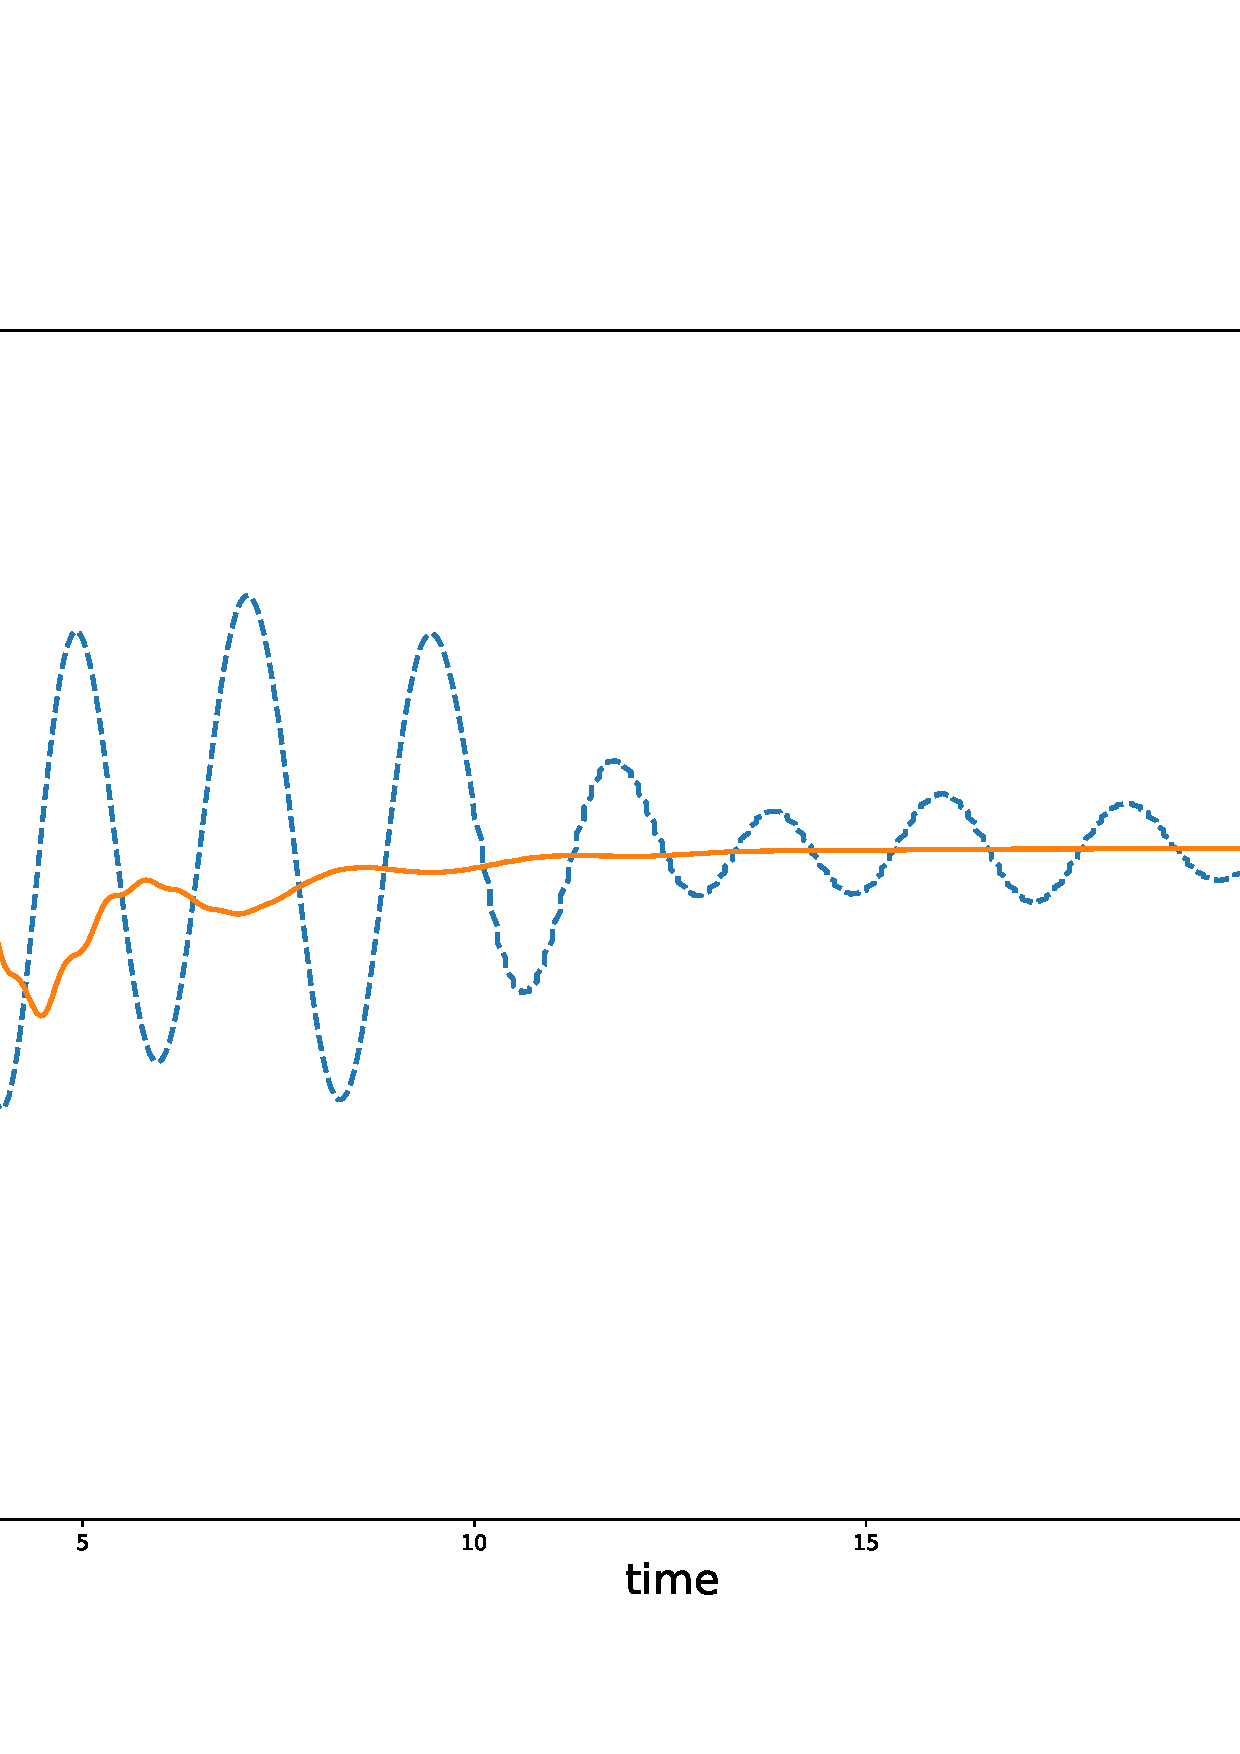
\includegraphics[scale=0.41]{theta.pdf}}
		\caption{Helicopter SMC and SAC Euler angles by initial position [-1,-1,-1].}
		\label{theta}
	\end{center}
\end{figure}

\begin{figure}
	\begin{center}
		{\includegraphics[scale=0.41]{V.pdf}}
		\caption{Helicopter SMC and SAC velocities by initial position [-1,-1,-1].}
		\label{v_res}
	\end{center}
\end{figure}

\begin{figure}
	\begin{center}
		{\includegraphics[scale=0.41]{col.pdf}}
		\caption{Helicopter SMC and SAC control input by initial position [-1,-1,-1].}
		\label{actions_delta}
	\end{center}
\end{figure}

\begin{figure}
	\begin{center}
		{\includegraphics[scale=0.41]{flapping.pdf}}
		\caption{Helicopter SMC and SAC flapping states by initial position [-1,-1,-1].}
		\label{flapping}
	\end{center}
\end{figure}